%\vspace{-.8cm}
\section{Introduction}
\label{sec:introduction}

The field of medical image segmentation has experienced transformative growth through the development of U-shaped convolutional neural network (CNN) architectures \cite{ronneberger2015u,oktay2018attention,zhou2018unet++,fan2020pranet} such as UNet \cite{ronneberger2015u}, UNet++ \cite{zhou2018unet++}, AttnUNet \cite{oktay2018attention}, PraNet \cite{fan2020pranet}, UACANet \cite{kim2021uacanet}, and DeepLabv3+ \cite{chen2017deeplab}. These models excel at segmenting medical images, enabling precise segmentation of critical tumors, lesions, or polyps. Attention mechanisms \cite{oktay2018attention,fan2020pranet,woo2018cbam} integrated into these architectures help refine feature maps, thus enhancing pixel-level classification. However, the substantial computational demands of these models, including those with attention mechanisms, limit their applicability in resource-constrained environments such as point-of-care diagnostics.

The introduction of vision transformers \cite{chen2021transunet,cao2021swin,rahman2024g,Rahman_2023_WACV,rahman2023multi,rahman2024emcad,valanarasu2021medical}, including TransUNet \cite{chen2021transunet}, SwinUNet \cite{cao2021swin} and MedT \cite{valanarasu2021medical}, marked a shift towards leveraging self-attention to capture long-range dependencies within images for a comprehensive global view. However, transformers tend to neglect crucial local spatial relationships among pixels which are essential for precise segmentation. Moreover, transformers usually have high memory and computational demands for calculation and fusing attention with convolutional mechanisms, which limits their practical deployment. 

%UNeXt \cite{valanarasu2022unext}, a lightweight architecture, bridges this gap by combining the strengths of CNNs and multi-layer perceptron (MLP), but faces challenges in precise segmentation. 
In recent years, a good number of lightweight architectures such as UNeXt \cite{valanarasu2022unext}, CMUNeXt \cite{tang2023cmunext}, MALUNet \cite{ruan2022malunet}, EGE-UNet \cite{ruan2023ege}, and Rolling-UNet \cite{liu2024rolling}, bridge this gap by combining the strengths of CNNs and multi-layer perceptron (MLP). However, most of these architectures are designed for less complex or easy-to-segment applications such as skin lesions, breast cancer in ultrasound, and microscopic cell nuclei/structure segmentation. Consequently, these architectures show poor performance in challenging applications like polyp segmentation due to the high variability in the shape, size, and texture of polyps.


\begin{figure*}[t]
\centering
%\vspace{-.2cm}
\begin{subfigure}{.45\textwidth}
  \centering
  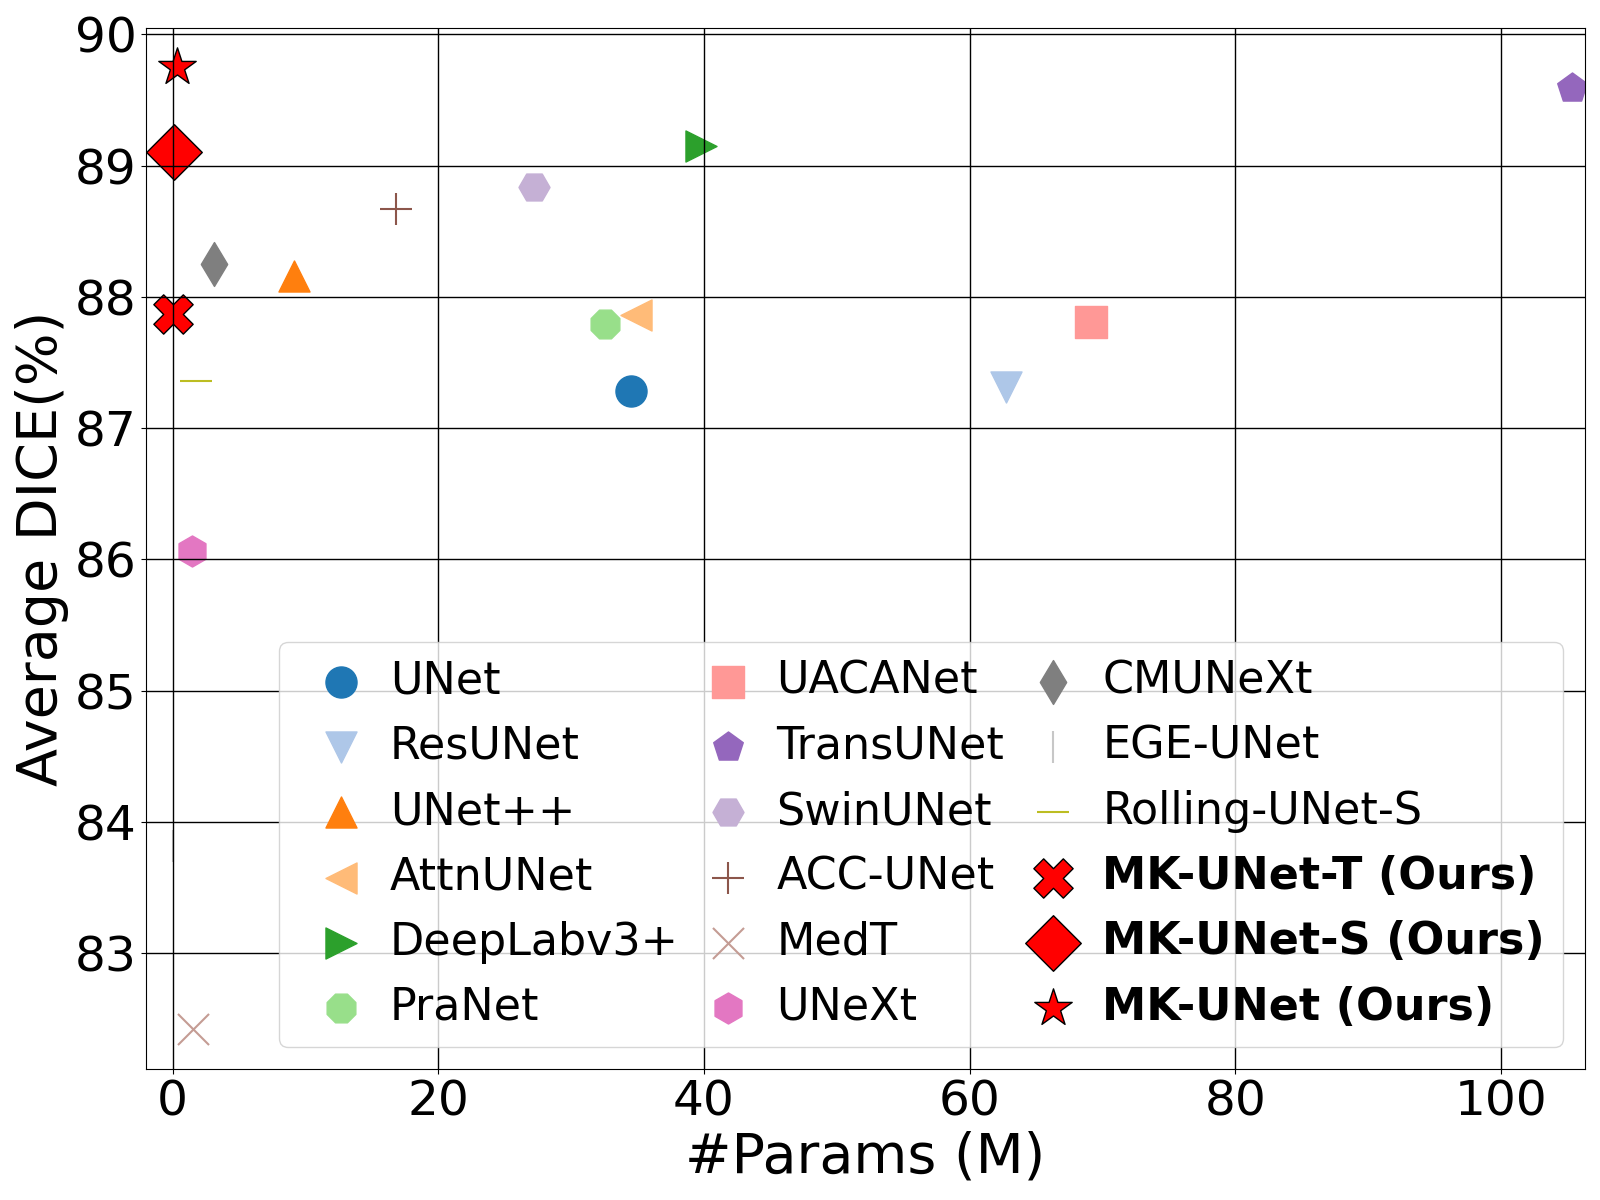
\includegraphics[width=1\linewidth]{sections/imgs/avg_dice_params_mkunet.png}
  %\vspace{-.25cm}
  \caption{Average DICE scores vs. \#Params}
  \label{fig:dice_vs_params}
\end{subfigure}%
\begin{subfigure}{.45\textwidth}
  \centering
  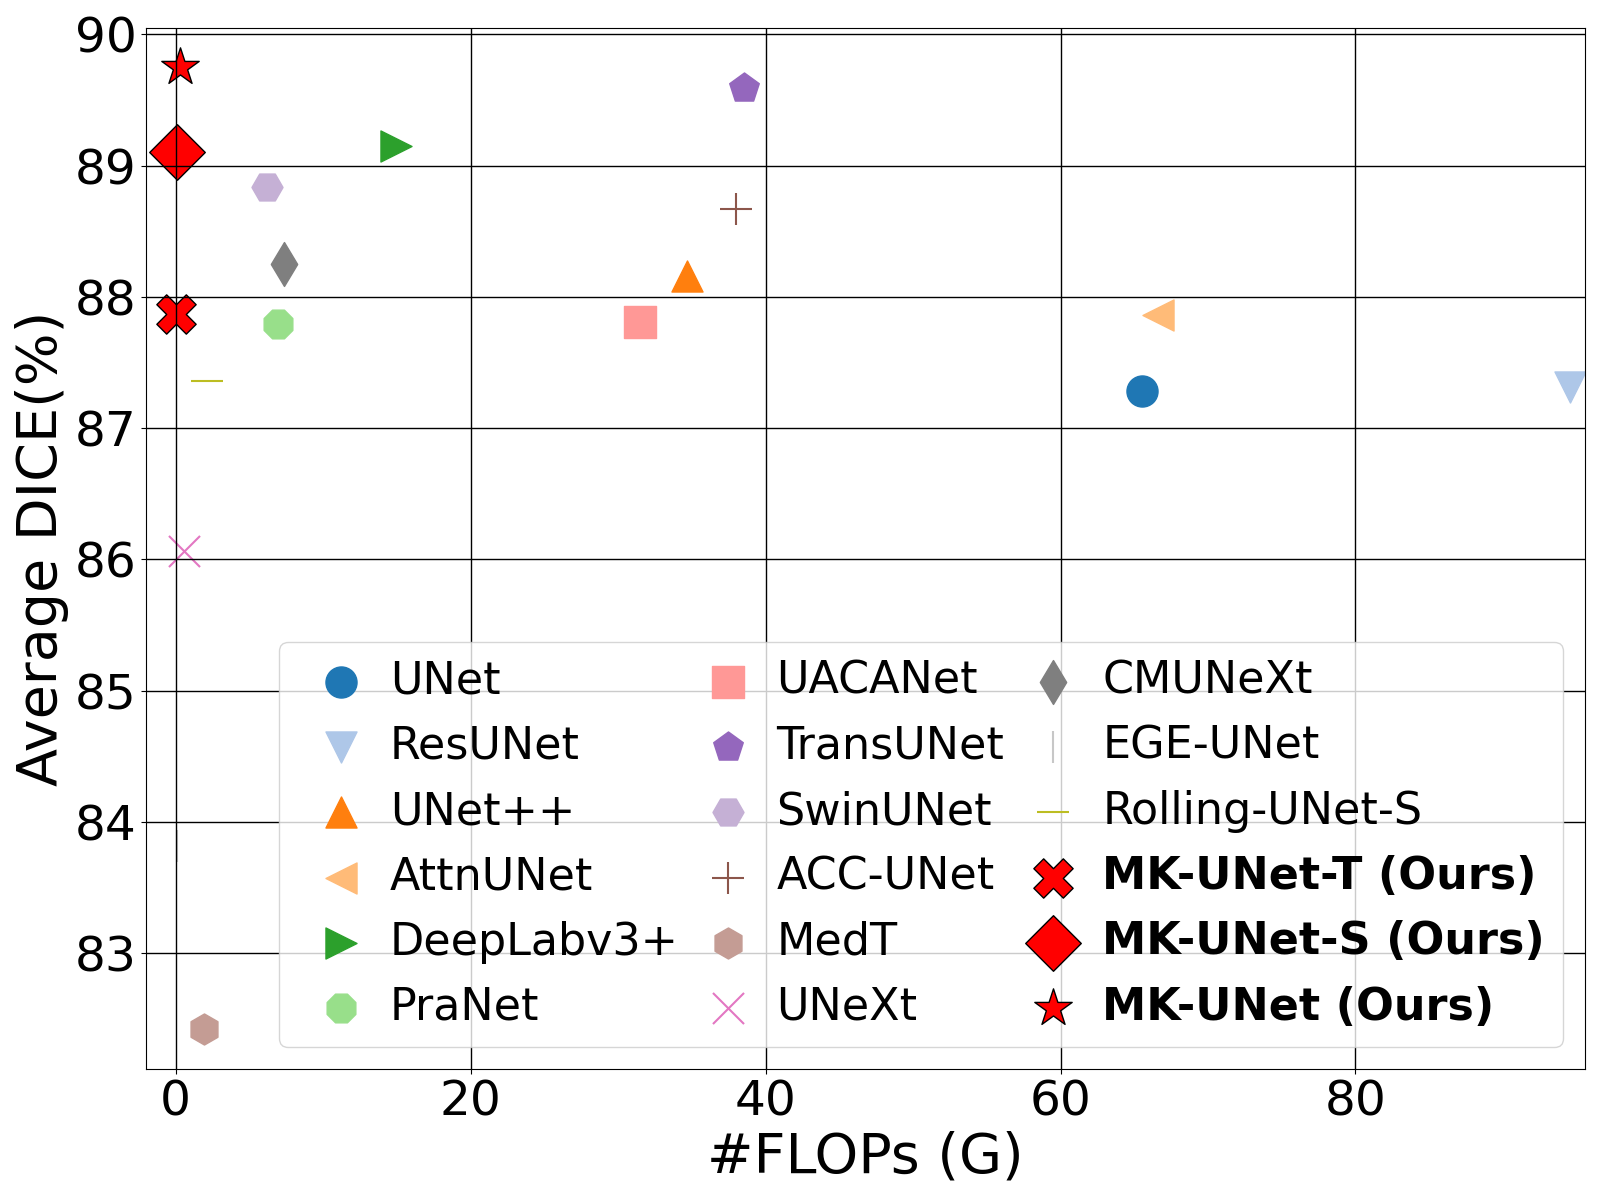
\includegraphics[width=1\linewidth]{sections/imgs/avg_dice_flops_mkunet.png}
  %\vspace{-.25cm}
  \caption{Average DICE scores vs. \#FLOPs}
  \label{fig:dice_vs_flops}
\end{subfigure}
\vspace{-.1cm}
\caption{Comparison of MK-UNet against different SOTA methods over six binary medical image segmentation datasets. As shown, our MK-UNet has the second lowest \#Params and \#FLOPs (behind EGE-UNet \cite{ruan2023ege}), yet the highest DICE scores. Though EGE-UNet has the lowest \#Params and \#FLOPs among existing methods, it has the lowest DICE score as well.}
\label{fig:dice_vs_params_flops}
\vspace{-.2cm}
\end{figure*}

%and optimization of computational resources.

To address these computational and precision challenges, we introduce MK-UNet, a significant breakthrough in image segmentation, which leverages the benefits of a multi-kernel perspective (i.e., $k_1=k_2$ or $k_1 \neq k_2$ for $k_1, k_2 \in Kernels$) and depth-wise convolutions to address the computational complexity and challenges inherent in existing CNN- and transformer-based models. Depth-wise convolutions drastically reduce the computational load, making the network more efficient without sacrificing the ability to capture detailed features within the image. Additionally, our multi-kernel property enables the model to effectively handle feature representations at \textit{same or varying} receptive fields, thus allowing for a more robust and comprehensive analysis of complex images in diverse applications. Moreover, by incorporating sophisticated convolutional multi-focal (channel and spatial) attention mechanisms \textit{only} in our decoder further refines the feature maps by capturing the image salient features. We note that our network is effective for segmentation in both scenarios, whether the regions of interest vary significantly in size and shape or remain relatively uniform. By integrating these new ideas, MK-UNet achieves a fine balance between computational efficiency and segmentation accuracy, thus offering an ultra-lightweight model that not only surpasses the performance of heavyweight counterparts (in DICE scores), but it does so with significantly fewer \#Params and \#FLOPs. Our contributions are as follows:

\begin{itemize}
%\vspace{-.2cm}
    \item \textbf{New Lightweight Multi-kernel UNet:} We propose a new end-to-end U-shaped network, MK-UNet, for medical image segmentation, which encodes an image using lightweight multi-kernel convolutions to capture multi-resolution spatial representations. MK-UNet also progressively refines the multi-resolution spatial representations using multi-kernel convolutional attention. Of note, our MK-UNet-T (tiny) has only 0.027M and 0.062G \#Params and \#FLOPs, respectively, yet provides SOTA performance. Moreover, MK-UNet (standard) has only 0.316M \#Params and 0.314G \#FLOPs. The extremely low model size (\#Params) and computations (\#FLOPs) make our MK-UNet easy to deploy in point-of-care diagnostics or resource-constraint environments (e.g., mobile or edge devices).
    \item \textbf{Lightweight Multi-kernel Inverted Residual:} We introduce MKIR, a new Multi-Kernel Inverted Residual block that performs depth-wise convolutions with multiple kernels (i.e., $k_1=k_2$ or $k_1 \neq k_2$, for $k_1, k_2 \in Kernels$). Our encoder extracts features using the MKIR block; this choice is motivated by the need to efficiently process and encode diverse and complex structures in medical images, thus providing a rich representation with minimal computational costs.
    \item \textbf{Lightweight Multi-kernel Inverted Residual Attention:} We propose Multi-Kernel Inverted Residual Attention (MKIRA), a new block to refine and enhance multi-scale salient features by suppressing irrelevant regions. In our decoder, MKIRA enhances features discrimination by focusing on key feature channels and highlighting the important spatial regions in an image. This ensures that the decoder can reconstruct precise and accurate segmentation maps by focusing only on the most critical aspects of the encoded features. 
    %\item \textbf{Lightweight Grouped Attention Gate:} We introduce a new grouped attention gate to combine refined features with skip connections. By using $3\times3$ group convolutions instead of point-wise convolutions, our attention gate captures salient features in a larger local context with less computation.
    \item \textbf{Improved Performance across Various Tasks and Benchmarks:} We empirically show that MK-UNet significantly improves the performance of medical image segmentation compared to SOTA methods with a significantly lower computational cost (as shown in Fig. \ref{fig:dice_vs_params_flops}) on six binary medical image segmentation benchmarks that belong to four different tasks.
\end{itemize}

The remaining of this paper is organized as follows: Section \ref{sec:method} describes the proposed method. Section \ref{sec:experiments} explains our experimental setup and results on six medical image segmentation benchmarks. Section \ref{sec:ablation_study} covers different ablation experiments. Lastly, Section \ref{sec:conclusion} concludes the paper. 
%-------------------------------------------------------------------------


